\chapter{Experimentation and results}
\label{Chapter4}

After having explained the necessary theoretical background and presented the proposals
of this work, it is time that we put them into action to see how they perform. First, we are going
to test our proposals on some toy datasets in order to better understand them. After that, we are going
to try the proposed invariants as well as the multiclass extension with ECOC on real data to see how
well they perform when comparing them to the original invariants proposed in \cite{Vapnik2019}.

\section{Experimenting with toy problems}

In this section we will perform a set of simple experiments with some toy datasets. In this case, we have
considered the circles and moons datasets, which can be seen in figure \ref{fig:toy_datasets}. Both of
these problems are available in \texttt{scikit-learn}, which means that we will be able to easily generate
our custom datasets with the available functions. When experimenting with these problems we aim to:

\begin{itemize}
    \item Compare the original invariants with the ones that have been proposed in this work.
    \item Compare the original version of the LUSI algorithm with the ECOC version to see if there is
    any significant difference in a binary setting.
    \item Discover whether some types of invariants are more likely to be selected when considering all types
    of invariants.
\end{itemize}

\begin{figure}[H]
    \centering
    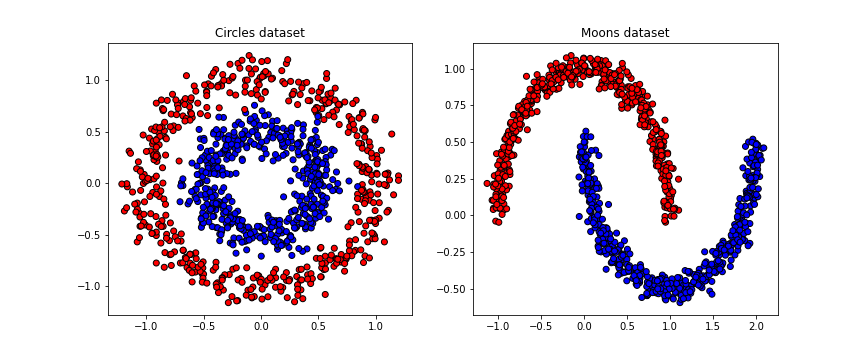
\includegraphics[width=\textwidth]{thesis/Figures/toy_datasets.png}
    \caption{Toy datasets used in the experimentation.}
    \label{fig:toy_datasets}
\end{figure}

For this experimentation, we have generated one dataset for each problem with a fixed seed. The experimental
parameter settings for each type of problem can be seen in table \ref{tab:toy_problems_experiments}. In an experiment,
we split the data in training and test, keeping 10\% of the data in the training partition and the reamining
90\% in the test partition. We have performed these experiments using Vapnik's invariants and the ones
that we have proposed. As for Vapnik's invariants, we have considered the zeroth and first order invariants, which are

\[
    \psi_0(x) = 1,\quad \psi_1(x) = x_1,\quad \psi_2(x) = x_2
\]

\subsection{Comparing the different invariant types and versions of LUSI}

In order to compare the two versions of the LUSI algorithm and the different invariants
we have trained a model for each version of LUSI and each invariant type on both problems with a fixed
initial random state. We have visualized the decision boundaries in each case in order to see if there is any
significant difference between them. Also, for the LUSI version we have reported the mean number of selected
invariants of each type by repeating the experiment with 10 different initial states. We have limited the
maximum number of invariants of each model to 3 because even though we can generate infinite new random
invariants, we cannot do the same with the original invariants.

\begin{table}[h]
\centering
\begin{tabular}{llr}
\textbf{Problem} & \textbf{Parameter}  & \textbf{Value} \\ \hline
Circles          & \texttt{n\_samples} & 1000           \\
                 & \texttt{noise}      & 0.1            \\
                 & \texttt{factor}     & 0.5            \\
Moons            & \texttt{n\_samples} & 1000           \\
                 & \texttt{noise}      & 0.05          
\end{tabular}
\caption{Parameter settings of the toy problems.}
\label{tab:toy_problems_experiments}
\end{table}

Figures \ref{fig:circles_decision_boundary} and \ref{fig:moons_decision_boundary} show the decision
boundaries generated by the original version of the LUSI algorithm whereas figures
\ref{fig:circles_decision_boundary_ecoc} and \ref{fig:moons_decision_boundary_ecoc} display the decision
boundaries of the ECOC version. For the circles problem, we can see that all invariants produce
very similar decision boundaries. In the case of ECOC version, this decision boundary seems to be much
closer to the points of the blue class than in the case of the original algorithm, where the decision boundary
is a bit wider. As for the moons problem, we can observe that the decision boundary is not perfect
in any of the versions of the algorithm since some points fall into the region of the opposite class,
probably caused by to the geometric shape of the both classes. For this problem, the decision boundary seems
to be more accurate using the original algorithm. This is especially true in the case of the random hyperplanes,
where the decision boundary is better adjusted in the case of the original algorithm, whereas it seems that it
has been overfitted when using the ECOC algorithm because we can observe some ``decision islands'' for the blue
class. Overall, it seems that Vapnik's invariants and the random projections produce very similar results
regardless of which version of the algorithm is applied. Hence, if we use any of these two invariants, we
could apply any version of the algorithm and get similar results in a binary classification problem. In the
case of the random hyperplanes, there would be some difference between the results obtained with each version
of the algorithm. As we have seen, depending on the problem, we could get similar results to the ones obtained
using the other two types of invariants.

The idea that Vapnik's invariants and the random projections are similar can be further explored. Figure
\ref{fig:toys_small_num_selected_invariants} show how many invariants have been selected for each problem
on average. We can observe that the mean number of selected invariants is the same for Vapnik's invariants
and the random projections, whereas the number of selected invariants is equal to the maximum number of
invariants in the case of the random hyperplanes. Thus, it seems that the number of invariants that can be
chosen when using Vapnik's invariants and the random projections is limited by the number of dimensions of the
data, as selecting more does not provide any new information. In the case of the random hyperplanes, this is
generally not true as we could keep adding more invariants of this type. This might be caused by the
fact that there is a very large number of hyperplanes that separate the data in two partitions and that
can be used to preserve the proportion of elements that fall on the right side of the hyperplane.
Because of this, many invariants of this type can be selected.

\subsection{Exploring the bias towards certain types of invariants}

Now, we would like to study the scenario in which all types of invariants are considered to see if there is
any kind of bias towards particular types of invariants. For this purpose, we have run a similar experiment to
the previous one using the original version of the LUSI algorithm. Using both problems, we have fit 10 models
using different random states and setting the maximum number of invariants to 50. In each experiment, the model could
choose among all of the invariant types. For each run, we have computed how many invariants of each
type were selected.

A summary of the results can be seen in figure \ref{fig:toys_mean_num_selected}, where the number of
selected invariants has been averaged for each problem. We can see that the models have not selected any of
Vapnik's invariants. On average, they have chosen 2 random projections per problem, which once again matches
the number of dimensions that these problems have. The models have selected 48 random hyperplanes on average
per problem, which gives more strength to the hypothesis that the number of hyperplane invariants that
can be selected is very large, potentially infinite. Because of this, we can see that when considering
all types of invariants at the same time, it is more likely that the hyperplanes invariant will be selected
because it can contribute with more information.

\begin{figure}[H]
    \centering
    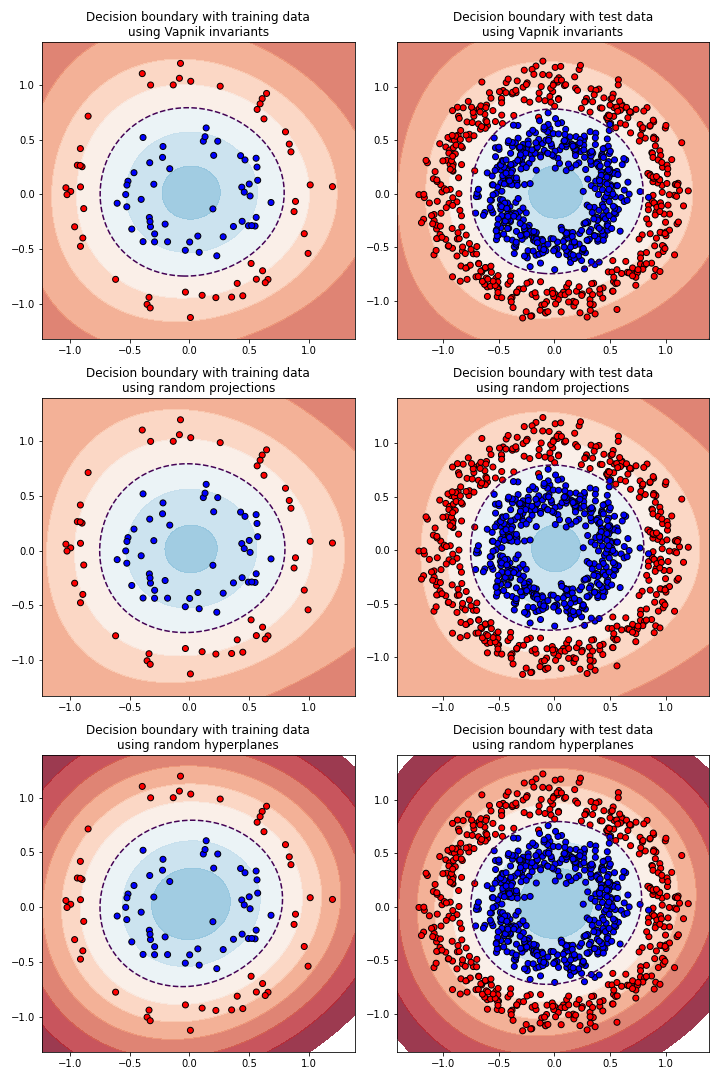
\includegraphics[width=\textwidth]{thesis/Figures/circles_decision_boundaries.png}
    \caption{Decision boundaries in the circles problem using the original LUSI algorithm with each type of
    invariant on the training and test sets.}
    \label{fig:circles_decision_boundary}
\end{figure}

\begin{figure}[H]
    \centering
    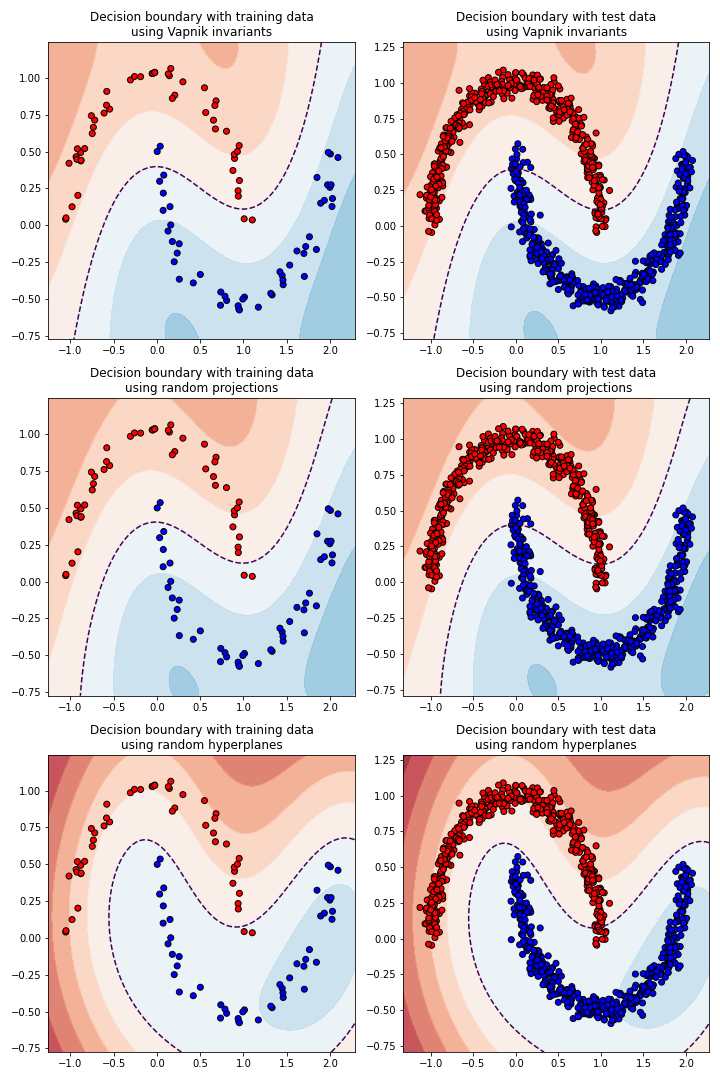
\includegraphics[width=\textwidth]{thesis/Figures/moons_decision_boundaries.png}
    \caption{Decision boundaries in the moons problem using the original LUSI algorithm with each type of
    invariant on the training and test sets.}
    \label{fig:moons_decision_boundary}
\end{figure}

\begin{figure}[H]
    \centering
    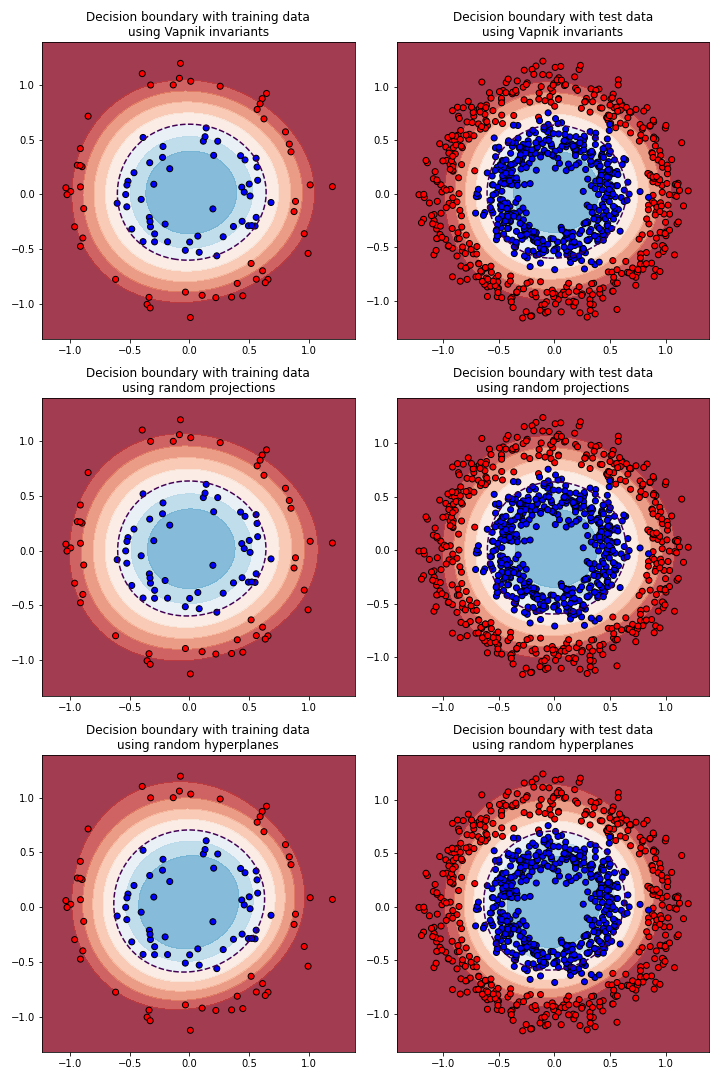
\includegraphics[width=\textwidth]{thesis/Figures/circles_decision_boundaries_ecoc.png}
    \caption{Decision boundaries in the circles problem using the ECOC version of the LUSI algorithm with each type
    of invariant on the training and test sets.}
    \label{fig:circles_decision_boundary_ecoc}
\end{figure}

\begin{figure}[h]
    \centering
    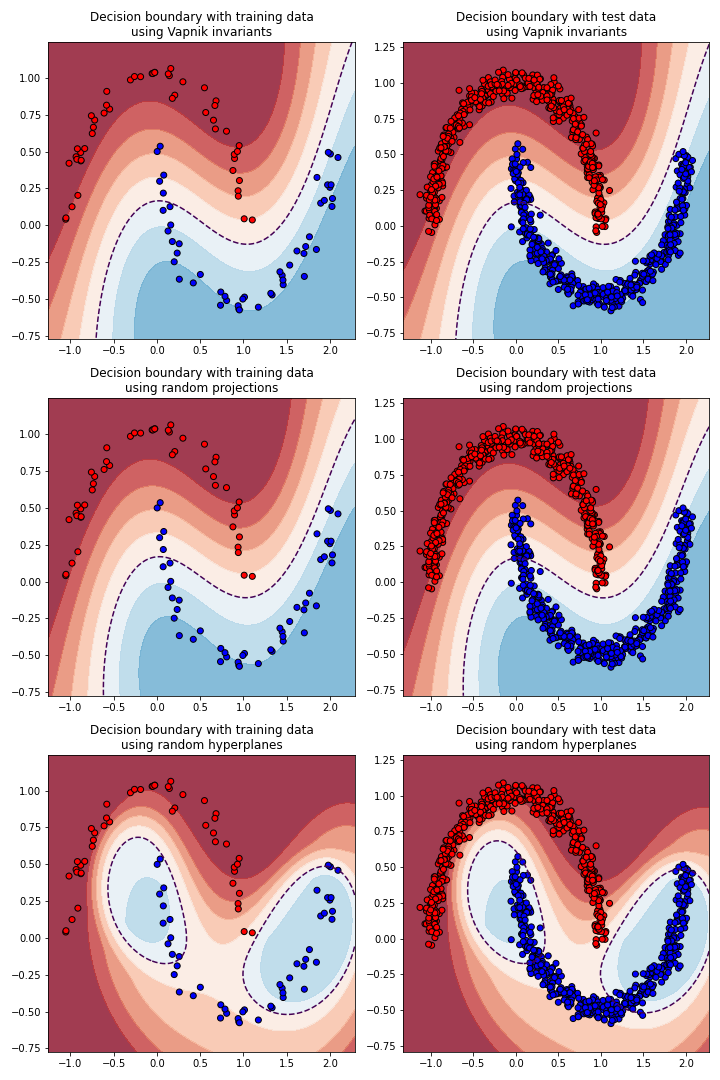
\includegraphics[width=\textwidth]{thesis/Figures/moons_decision_boundaries_ecoc.png}
    \caption{Decision boundaries in the moons problem using the ECOC version of the LUSI algorithm with each type
    of invariant on the training and test sets.}
    \label{fig:moons_decision_boundary_ecoc}
\end{figure}

\begin{figure}[H]
    \centering
    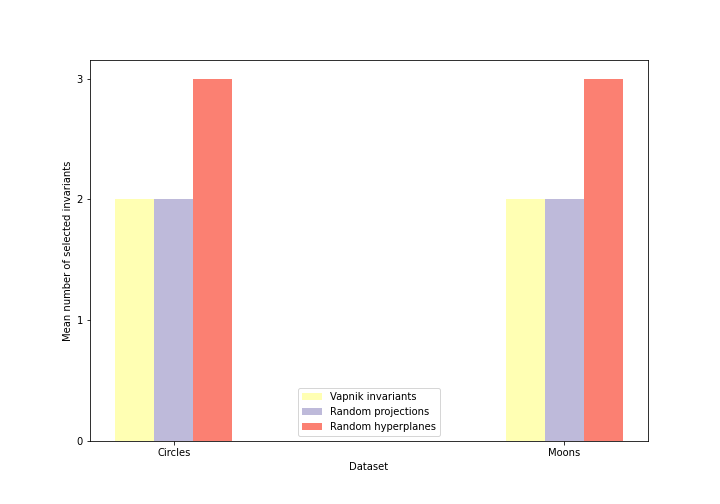
\includegraphics[width=0.8\textwidth]{thesis/Figures/num_selected_invariants.png}
    \caption{Mean number of selected invariants per problem. The maximum number of invariants was set to 3.}
    \label{fig:toys_small_num_selected_invariants}
\end{figure}

\begin{figure}[H]
    \centering
    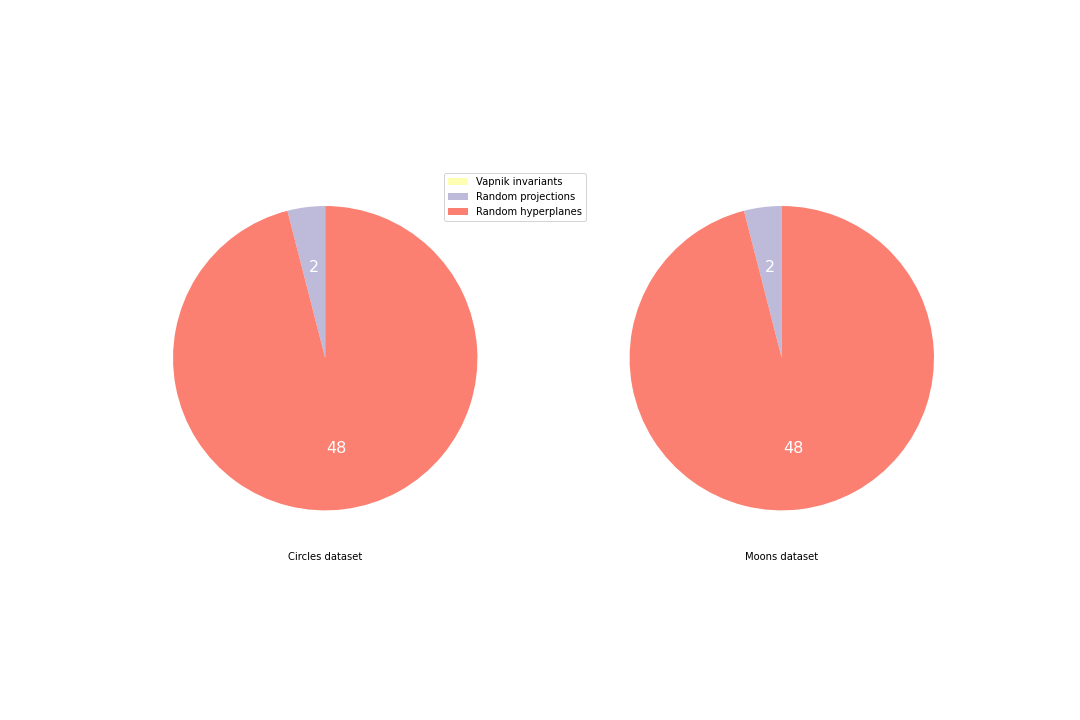
\includegraphics[width=\textwidth]{thesis/Figures/mean_num_selected.png}
    \caption{Mean number of selected invariants when the maximum number of invariants is 50 and the three types of
    invariants are considered simultaneously.}
    \label{fig:toys_mean_num_selected}
\end{figure}

\section{Experimentation on real data}

Once we have got a glimpse of how the proposals compare to the original work, we would like to test them
on real problems to see how they perform compared to the base version.

\subsection{Experimental settings}
{\bf Data:} Datos y tabla resumen de los datasets\\
{\bf Baselines:} Que métodos vas a comparar.
SVM sin invariantes
SVM con invariantes Vapnik
SVM con invariantes Vladis

Todos con el mismo sistema de selección.
\\
{\bf Methodology and performance metrics:} XValidation? cuanto, como mides los resultados?

Accuracy promedio i desviación estandar.
\\
{\bf Experimental and parameter setting:}
Haces parameter tunning?

Que experimentos propones?

1- Experimento base: Todos los datos con los modelos a comparar\\
2- Experimento con reduccion de datos.

\begin{table}[H]
\centering
\begin{tabular}{lrrr}
\textbf{Problem} & \textbf{Num. examples} & \textbf{Attributes} & \textbf{Classes} \\ \hline
Balance scale    & 625                    & 4                   & 3                \\
Ecoli            & 336                    & 8                   & 8                \\
Glass            & 214                    & 9                   & 7(6)\tablefootnote{According to the dataset's documentation, there are 7 classes. However, there is one that does not have any elements. Therefore, the actual number of classes for this problem is 6.}                \\
Iris             & 150                    & 4                   & 3                \\
Yeast            & 1484                   & 8                   & 10              
\end{tabular}
\caption{Caption}
\label{tab:problems_description}
\end{table}


\subsection{Results}

% Please add the following required packages to your document preamble:
% \usepackage{graphicx}
\begin{table}[h]
\centering
\resizebox{\textwidth}{!} &
  10\% &
  \multicolumn{1}{c|}{100\%} &
  10\% &
  \multicolumn{1}{c|}{100\%} &
  10\% &
  \multicolumn{1}{c|}{100\%} &
  10\% \\ \hline
\multicolumn{1}{|c|}{Balance scale} &
  \multicolumn{1}{c|}{$91.47 \pm 0.38\%$} &
  $88.80 \pm 1.73\%$ &
  \multicolumn{1}{c|}{$91.47 \pm 0.38\%$} &
  $87.73 \pm 2.10\%$ &
  \multicolumn{1}{c|}{$91.73 \pm 0.38\%$} &
  $83.73 \pm 7.17\%$ &
  \multicolumn{1}{c|}{$90.13 \pm 1.51\%$} &
  $76.00 \pm 12.77\%$ \\ \hline
\multicolumn{1}{|c|}{Ecoli} &
  \multicolumn{1}{c|}{$85.29 \pm 2.08\%$} &
  $71.57 \pm 1.39\%$ &
  \multicolumn{1}{c|}{$85.29 \pm 1.20\%$} &
  $72.55 \pm 4.22\%$ &
  \multicolumn{1}{c|}{$84.15 \pm 2.05\%$} &
  $67.32 \pm 4.03\%$ &
  \multicolumn{1}{c|}{$75.98 \pm 6.28\%$} &
  $63.89 \pm 9.61\%$ \\ \hline
\multicolumn{1}{|c|}{Glass} &
  \multicolumn{1}{c|}{$72.87 \pm 7.91\%$} &
  $56.59 \pm 4.78\%$ &
  \multicolumn{1}{c|}{$72.87 \pm 7.91\%$} &
  $45.74 \pm 6.67\%$ &
  \multicolumn{1}{c|}{$72.09 \pm 7.44\%$} &
  $52.45 \pm 7.03\%$ &
  \multicolumn{1}{c|}{$71.06 \pm 7.60\%$} &
  $45.48 \pm 9.50\%$ \\ \hline
\multicolumn{1}{|c|}{Iris} &
  \multicolumn{1}{c|}{$96.67 \pm 0.00\%$} &
  $93.33 \pm 2.72\%$ &
  \multicolumn{1}{c|}{$95.56 \pm 1.57\%$} &
  $90.00 \pm 4.71\%$ &
  \multicolumn{1}{c|}{$95.19 \pm 1.66\%$} &
  $77.78 \pm 22.93\%$ &
  \multicolumn{1}{c|}{$88.52 \pm 11.56\%$} &
  $84.81 \pm 9.04\%$ \\ \hline
\multicolumn{1}{|c|}{Yeast} &
  \multicolumn{1}{c|}{$53.76 \pm 1.04\%$} &
  $47.92 \pm 2.08\%$ &
  \multicolumn{1}{c|}{$53.87 \pm 1.20\%$} &
  $47.92 \pm 2.14\%$ &
  \multicolumn{1}{c|}{$52.53 \pm 5.44\%$} &
  $45.68 \pm 4.60\%$ &
  \multicolumn{1}{c|}{$50.39 \pm 5.33\%$} &
  $37.82 \pm 7.92\%$ \\ \hline
\end{tabular}%
}
\caption{Caption}
\label{tab:results_accuracies_errors}
\end{table}

\begin{figure}
    \centering
    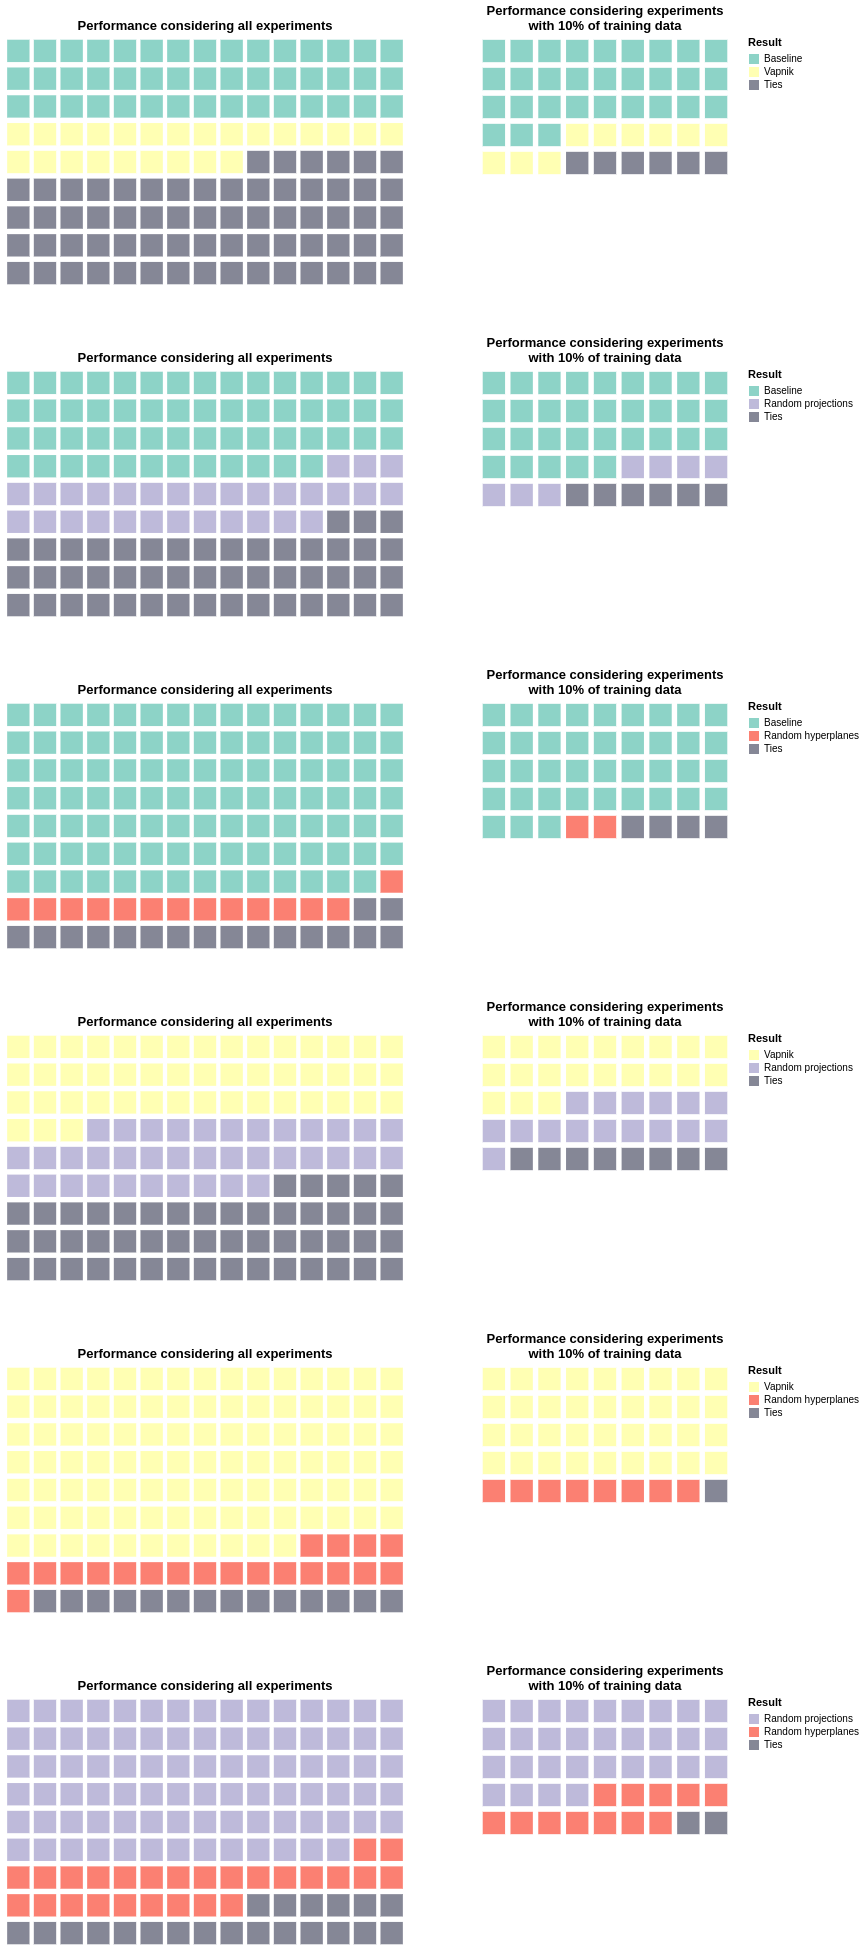
\includegraphics[width=0.7\textwidth]{thesis/Figures/invariants_performance.png}
    \caption{Caption}
    \label{fig:invariants_performance}
\end{figure}